\documentclass[UTF8]{ctexart}
\usepackage[margin=1in]{geometry}
\usepackage{amsmath}
\usepackage{amssymb}
\usepackage{listings}
\usepackage{xcolor}
\usepackage{graphicx}
\usepackage{tikz}
\usetikzlibrary{arrows.meta,positioning}
\usepackage{hyperref}
\usepackage{algorithmic}
\usepackage{algorithm}

% 代码格式设置(与其他章节保持一致)
\lstset{
		language=C++,
		basicstyle=\ttfamily\small,
		breaklines=true,
		numbers=left,
		numberstyle=\tiny,
		keywordstyle=\color{blue},
		commentstyle=\color{gray},
		stringstyle=\color{red},
		showstringspaces=false,
		backgroundcolor=\color{lightgray!20},
		frame=single
}

\title{AVL 树 (AVL Tree)}
\author{}
\date{}

\begin{document}

\maketitle

\section{AVL 树简介}
AVL 树是一种自平衡的二叉搜索树(Binary Search Tree,BST),由 Adelson-Velsky 和 Landis 在 1962 年提出。对于任意节点,AVL 树要求其左右子树的高度差(平衡因子,Balance Factor)至多为 1。通过在插入或删除后对局部子树做旋转来维护平衡,从而保证查找、插入、删除操作的时间复杂度为 $O(\log n)$。

\subsection{平衡因子 (Balance Factor)}
定义:对于节点 $v$,平衡因子 $BF(v)=\text{height}(v.left)-\text{height}(v.right)$。AVL 要求 $BF(v)\in\{-1,0,1\}$ 对所有节点成立。

\section{四种旋转类型}
当某个节点失衡($|BF|>1$)时,可以根据失衡的方向选择以下四种旋转之一来恢复平衡:\newline

1. LL(Left-Left)— 对左子树的左侧插入导致的失衡,使用单次右旋(RightRotate)修正。
2. RR(Right-Right)— 对右子树的右侧插入导致的失衡,使用单次左旋(LeftRotate)修正。
3. LR(Left-Right)— 对左子树的右侧插入导致的失衡,先对左子节点做左旋,再对当前节点做右旋(双旋)。

4. RL(Right-Left)— 对右子树的左侧插入导致的失衡,先对右子节点做右旋,再对当前节点做左旋(双旋)。

为了更直观地理解,每种旋转下给出图示(左侧为旋转前,右侧为旋转后):

\subsection*{LL (单次右旋) 图示}
\begin{center}
\begin{tikzpicture}[level distance=12mm, sibling distance=18mm, every node/.style={circle,draw,inner sep=1.5pt}]
	% before
	\node (y) {y}
		child { node (x) {x}
			child { node (z) {z} }
			child [missing] {}
		}
		child [missing] {};
	% arrow
	\node[right=2.6cm of y] (arrow) {\large $\Rightarrow$};
	% after
	\node[right=4.2cm of y] (x2) {x}
		child { node (z2) {z} }
		child { node (y2) {y} };
\end{tikzpicture}
\end{center}

\subsection*{RR (单次左旋) 图示}
\begin{center}
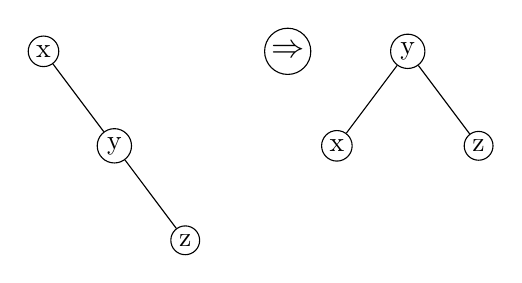
\begin{tikzpicture}[level distance=12mm, sibling distance=18mm, every node/.style={circle,draw,inner sep=1.5pt}]
	% before
	\node (x) {x}
		child [missing] {}
		child { node (y) {y}
			child [missing] {}
			child { node (z) {z} }
		};
	% arrow
	\node[right=2.6cm of x] (arrow2) {\large $\Rightarrow$};
	% after
	\node[right=4.2cm of x] (y2) {y}
		child { node (x2) {x} }
		child { node (z2) {z} };
\end{tikzpicture}
\end{center}

\subsection*{LR (双旋:先左旋再右旋) 图示}
\begin{center}
\begin{tikzpicture}[level distance=12mm, sibling distance=18mm, every node/.style={circle,draw,inner sep=1.5pt}]
	% before
	\node (z) {z}
		child { node (y) {y}
			child [missing] {}
			child { node (x) {x} }
		}
		child [missing] {};
	% arrow
	\node[right=2.6cm of z] (arrow3) {\large $\Rightarrow$};
	% after (after double rotation)
	\node[right=4.2cm of z] (x2) {x}
		child { node (y2) {y} }
		child { node (z2) {z} };
\end{tikzpicture}
\end{center}

\subsection*{RL (双旋:先右旋再左旋) 图示}
\begin{center}
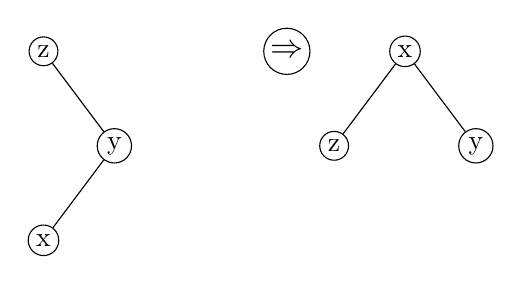
\begin{tikzpicture}[level distance=12mm, sibling distance=18mm, every node/.style={circle,draw,inner sep=1.5pt}]
	% before
	\node (z) {z}
		child [missing] {}
		child { node (y) {y}
			child { node (x) {x} }
			child [missing] {}
		};
	% arrow
	\node[right=2.6cm of z] (arrow4) {\large $\Rightarrow$};
	% after
	\node[right=4.2cm of z] (x2) {x}
		child { node (z2) {z} }
		child { node (y2) {y} };
\end{tikzpicture}
\end{center}

下面给出旋转的伪代码(方式 1:明确定义旋转操作并用于插入/删除恢复):

\begin{algorithm}
\caption{右旋(RightRotate)}
\begin{algorithmic}
\STATE \textbf{function} RightRotate(y)
		\STATE x $\leftarrow$ y.left
		\STATE T2 $\leftarrow$ x.right
		\STATE x.right $\leftarrow$ y
		\STATE y.left $\leftarrow$ T2
		\COMMENT{更新高度(假定有 UpdateHeight 函数)}
		\STATE UpdateHeight(y)
		\STATE UpdateHeight(x)
		\STATE \textbf{return} x
\ENDSTATE
\end{algorithmic}
\end{algorithm}

\begin{algorithm}
\caption{左旋(LeftRotate)}
\begin{algorithmic}
\STATE \textbf{function} LeftRotate(x)
		\STATE y $\leftarrow$ x.right
		\STATE T2 $\leftarrow$ y.left
		\STATE y.left $\leftarrow$ x
		\STATE x.right $\leftarrow$ T2
		\STATE UpdateHeight(x)
		\STATE UpdateHeight(y)
		\STATE \textbf{return} y
\ENDSTATE
\end{algorithmic}
\end{algorithm}

\subsection{插入时的重平衡伪代码}
\begin{algorithm}
\caption{AVL 插入(含重平衡)}
\begin{algorithmic}
\STATE \textbf{function} Insert(node, key)
		\IF{node is null}
				\STATE node $\leftarrow$ new Node(key)
				\STATE \textbf{return} node
		\ENDIF
		\IF{key < node.key}
				\STATE node.left $\leftarrow$ Insert(node.left, key)
		\ELSIF{key > node.key}
				\STATE node.right $\leftarrow$ Insert(node.right, key)
		\ELSE
				\STATE \textbf{return} node  \COMMENT{不允许重复键(或可按策略处理)}
		\ENDIF

		\STATE UpdateHeight(node)
		\STATE bf $\leftarrow$ Height(node.left) - Height(node.right)

		\COMMENT{LL 情形}
		\IF{bf > 1 AND key < node.left.key}
				\STATE \textbf{return} RightRotate(node)
		\ENDIF

		\COMMENT{RR 情形}
		\IF{bf < -1 AND key > node.right.key}
				\STATE \textbf{return} LeftRotate(node)
		\ENDIF

		\COMMENT{LR 情形}
		\IF{bf > 1 AND key > node.left.key}
				\STATE node.left $\leftarrow$ LeftRotate(node.left)
				\STATE \textbf{return} RightRotate(node)
		\ENDIF

		\COMMENT{RL 情形}
		\IF{bf < -1 AND key < node.right.key}
				\STATE node.right $\leftarrow$ RightRotate(node.right)
				\STATE \textbf{return} LeftRotate(node)
		\ENDIF

		\STATE \textbf{return} node
\ENDSTATE
\end{algorithmic}
\end{algorithm}

\section{具体示例}
下面给出一个简单的插入示例,演示 RR(右-右)失衡的修正过程(插入顺序:10, 20, 30):

\begin{enumerate}
	\item 插入 10:树为单节点 10。
	\item 插入 20:20 大于 10,成为 10 的右子节点。此时树为:
\begin{verbatim}
	10
		\\
		 20
\end{verbatim}
	\item 插入 30:30 比 10 和 20 都大,作为 20 的右子节点,形成右斜链:
\begin{verbatim}
	10
		\\
		 20
			 \\
				30
\end{verbatim}
	现在根节点 10 的平衡因子为 -2(高度差超过 1),且在其右子树的右侧插入(即 RR 情形),应对 10 做一次左旋(LeftRotate):

	左旋后结果为:
\begin{verbatim}
		 20
		/  \\
	10    30
\end{verbatim}
	经过左旋,树重新平衡,各节点的高度和 BF 均满足 AVL 要求。
\end{enumerate}

\section{小结}
\begin{itemize}
	\item AVL 树通过维护每个节点的高度并在必要时进行旋转,保证了操作的对数时间复杂度。
	\item 四种旋转(LL、RR、LR、RL)覆盖了所有可能的局部失衡情形。
	\item 示例展示了 RR 情形如何通过一次左旋恢复平衡。
\end{itemize}

\end{document}

